%! Author = tstreule

\section{Detection and Noise}
%%%%%%%%%%%%%%%%%%%%%%%%%%%%%%%%%%%%%%%%%%%%%%%%%%%%%%
%%%%%%%%%%%%%%%%%%%%%%%%%%%%%%%%%%%%%%%%%%%%%%%%%%%%%%
\subsection{Signal}
%
For statistically independent, ``uncorrelated'', events we use\\
\begin{minipage}{.3\columnwidth}
    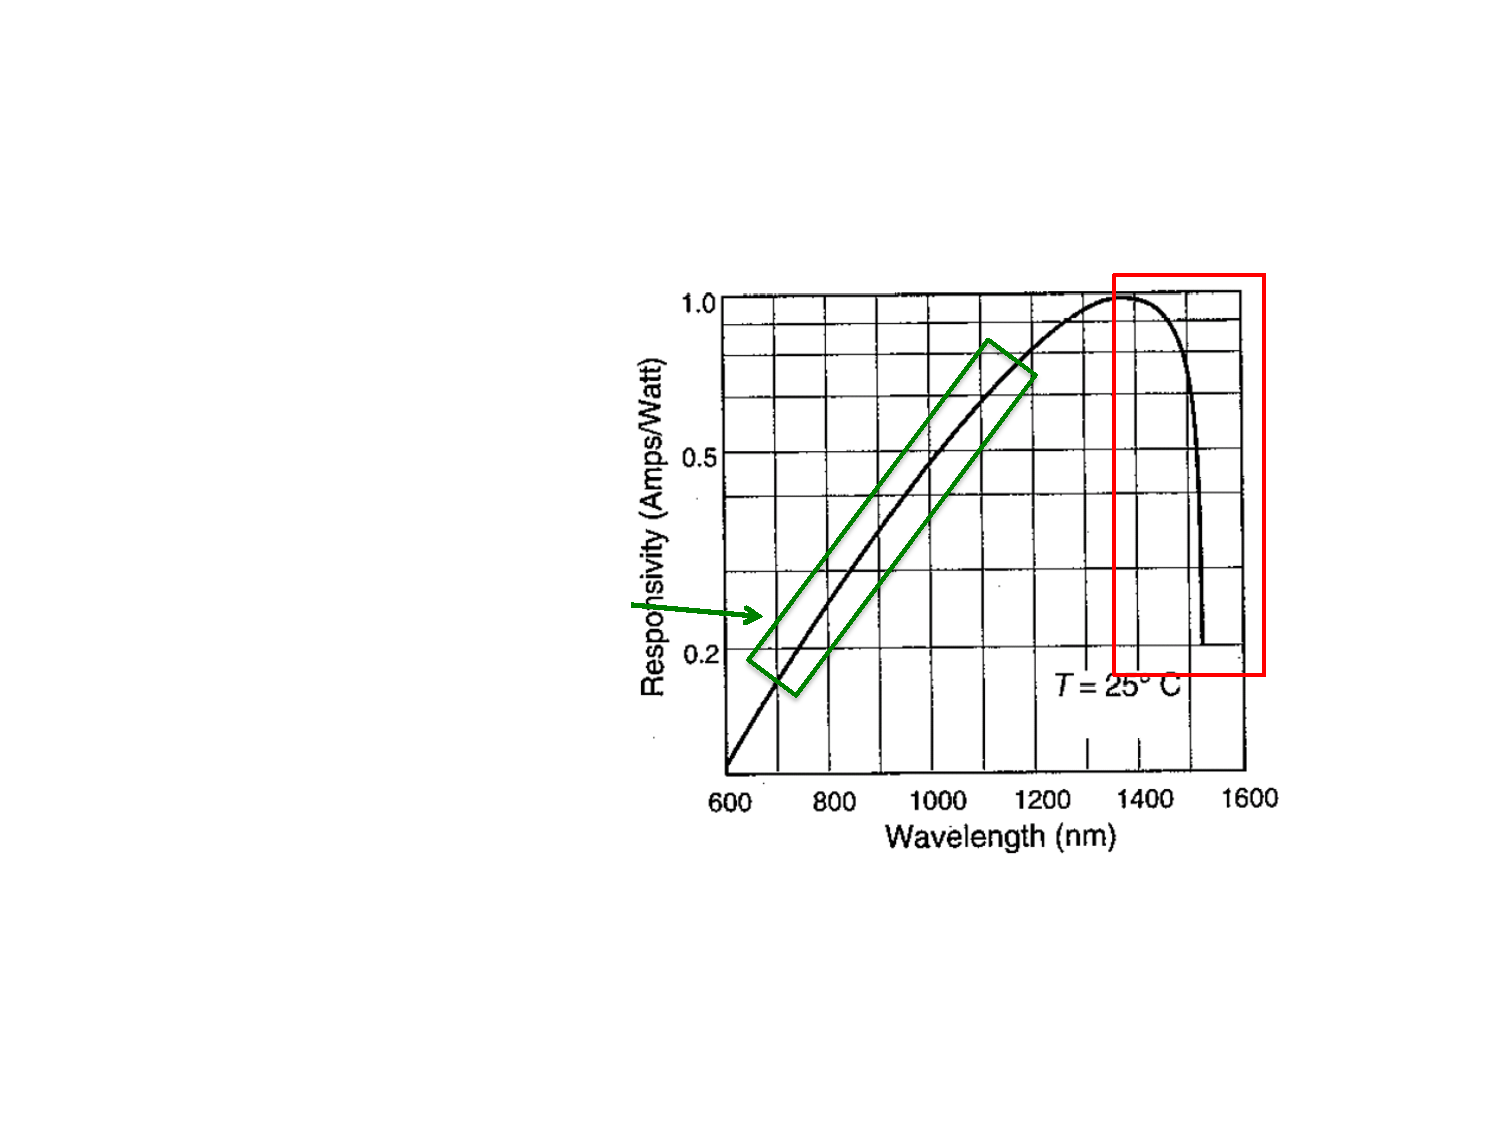
\includegraphics[width=.9\columnwidth]{Noise_QE_and_Responsivity}
\end{minipage}%
\begin{minipage}{.7\columnwidth}
    \formbox{\textbf{Poisson}}{P_{\overline{n}}(n)= \frac{\overline{n}^n}{n!} \eu^{-\overline{n}}}
    \parbox{.25\columnwidth}{$\overline{n}$: mean\\$\sigma_n \!=\! \sqrt{\overline{n}}$: var}
    \formula{Signal current}{\avg{I\ped{sig}} = \eta q\overline{n}/\Delta t}
    \formula{\textcolor[rgb]{0.23,0.49,0.14}{Responsivity}}{\avg{I\ped{sig}}/P = \eta q\lambda/(hc)}
    \formula{\textcolor{red}{Cutoff $\lambda$}}{\lambda(\unit{\mu m}) = 1.24/E(\unit{eV})}
\end{minipage}
%%%%%%%%%%%%%%%%%%%%%%%%%%%%%%%%%%%%%%%%%%%%%%%%%%%%%%
\subsubsection{Fundamental Noise Sources}
%
\formula{Noise\hfill \textbf{shot}}{N\ped{s} = 2R\eta qB \avg{I\ped{sig}} = \avg{I\ped{shot}^2} R \;,}
$2B \simeq 1/\Delta t$
\formula{\hfill \textbf{dark}}{N\ped{d} = 2R\eta qB \avg{I\ped{dark}}}
\vspace{-2mm}
\formula{\hfill thermal}{N\ped{J} = \avg{I\ped{Johnson}^2} R = \sqrt{\frac{k\ped{B}TB}{R}}^2 R}
\formula{\hfill \textbf{readout}}{N\ped{r} = N\ped{J}+N\ped{amplifier}}
\formbox{~}{N\ped{tot} = N\ped{s}+N\ped{d}+N\ped{r}}
$\sigma\ped{tot}^2 = \sum \sigma_i^2$
\formbox{SNR}{\textrm{SNR}\ped{curr} = \frac{\eta\cdot N_\gamma}{\sqrt{ \eta N_\gamma + N_d + N_r }}}
$\eta = \textrm{QE} \cdot absorb$
\formula{\centering for large numbers}{\textrm{SNR}\ped{shot} = \frac{\overline{n}}{\sqrt{\overline{n}}} = \sqrt{\overline{n}} \;\;\widehat{=}\;\; \eta N_\gamma}
%%%%%%%%%%%%%%%%%%%%%%%%%%%%%%%%%%%%%%%%%%%%%%%%%%%%%%
\subsection{(Optical) Detectors}
%
%	Characterizing Photodetectors
%	\begin{enumerate}
%		\item Quantum Eff.:
%			probability of generating a photoelectron
%		\item Internal Amplification:
%			ratio for converting a photoelectron into an output current
%		\item Dynamic Range:
%			largest and lowest (linearly) measurable signal
%		\item Response Speed:
%			$\Delta t$ and spread between incoming photon and output current burst
%		\item Geom. form factor:
%			Size and shape of the active area and the detector
%		\item Noise:
%			Shot noise vs. read-out noise dominated
%	\end{enumerate}
%
\formbox{\textbf{Photoel. effect}}{E\ped{ph} = hf = hc/\lambda = \phi + E\ped{kin}}
\formtex{~}{incident $E\ped{ph}$ = $E\ped{binding}$+$E\ped{kin}$ of ejected el.}
\formbox{Photo mult. (PMT)}{I = \alpha\;(S\cdot E\ped{ph}\,n/\Delta t) \;,}
$S$: sensitivity, $N\ped{d}\uparrow$

Choose \textbf{binning mode} (2x2, 4x4, …) such that the pixel size of the camera fits the best the maximum pixel size.
\formbox{\textbf{max. pixel size}}{\textrm{max} = 0.3 \frac{\lambda}{\textrm{NA}} \times M}\\
%%%%%%%%%%%%%%%%%%%%%%%%%%%%%%%%%%%%%%%%%%%%%%%%%%%%%%
%	\begin{center}
%		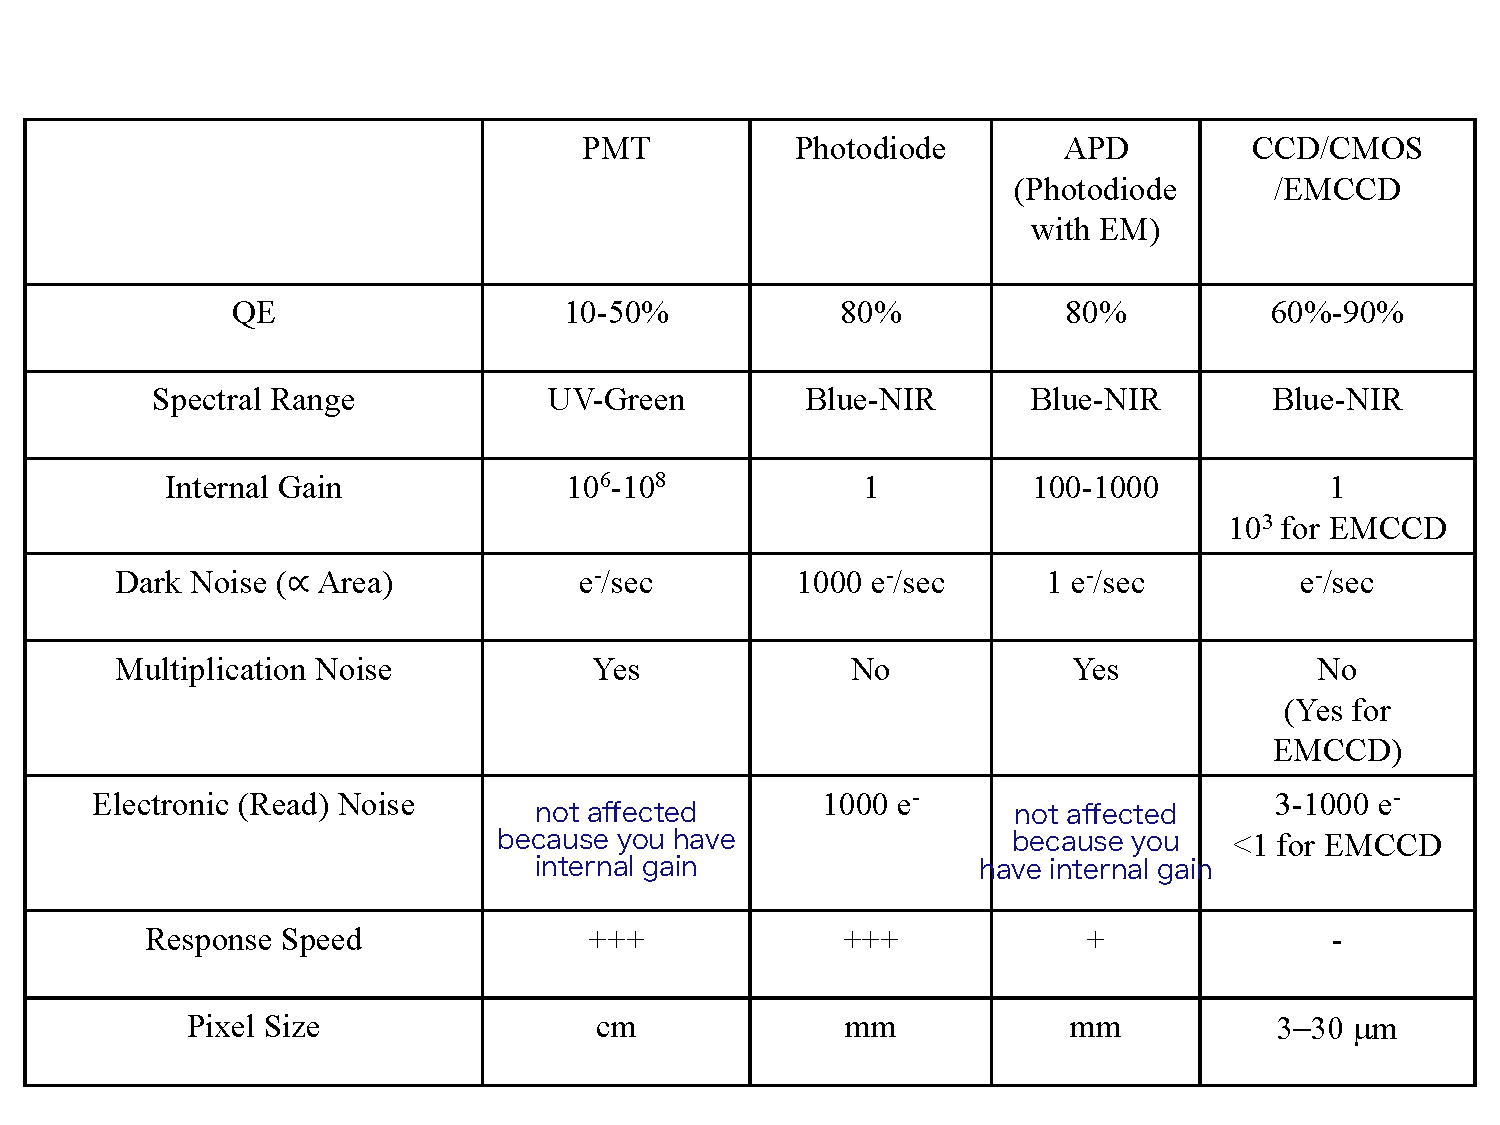
\includegraphics[width=.8\columnwidth]{Detection_Comparison}
%	\end{center}
%%%%%%%%%%%%%%%%%%%%%%%%%%%%%%%%%%%%%%%%%%%%%%%%%%%%%%
\subsection{Imaging Deep Tissues}
%
%	\textbf{Thick sample}: light will scatter, illuminating parts don't want to: SNR$\downarrow$
\formbox{Beer-Lambert's law}{I = I_0\,\eu^{-\mu\,x}}

\begin{minipage}{.5\columnwidth}
    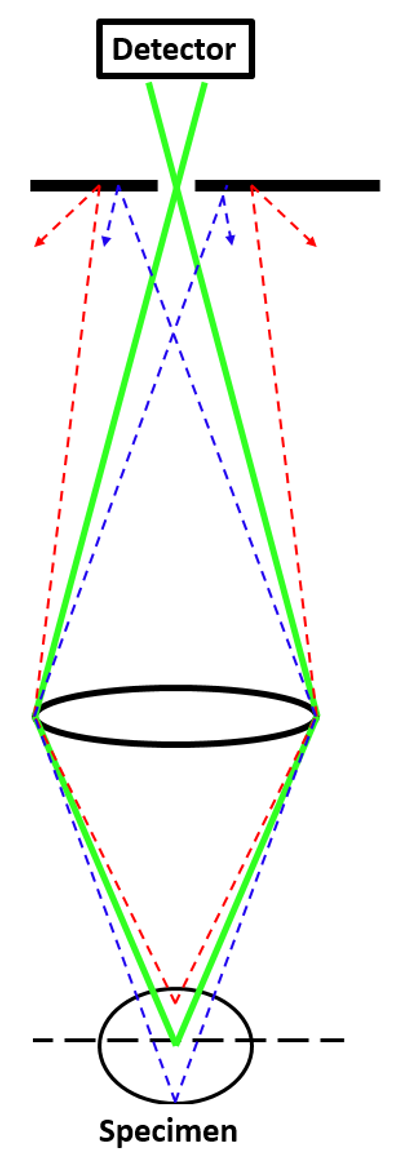
\includegraphics[width=.2\columnwidth]{Detection_Confocal_2}%
    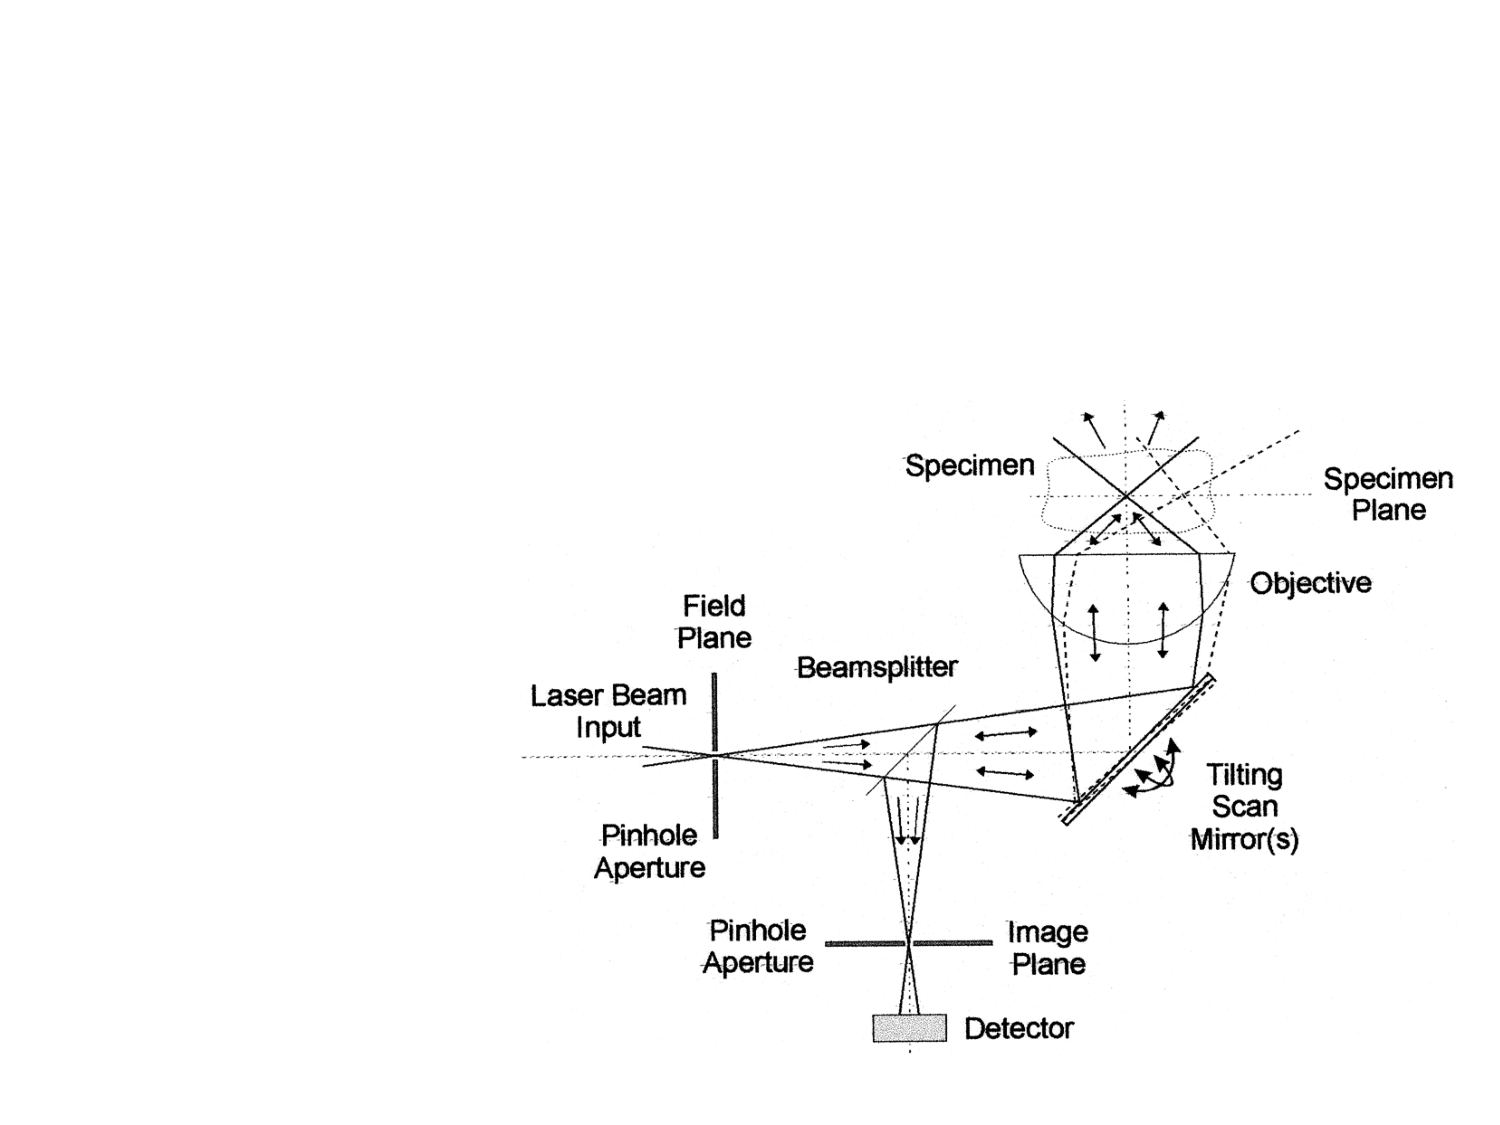
\includegraphics[width=.75\columnwidth]{Detection_Confocal_1}
\end{minipage}%
\begin{minipage}{.5\columnwidth}
    \textbf{1st} Pinhole by illumination:\\
    $\to$ focus the illum. to a small spot

    \textbf{2nd} Pinhole by detector:\\
    $\to$ reject out of focus light\\
    $\to$ collect light to PMT

    Signal and Noise (\textbf{Pinhole size}):\\
    $\bullet$ more out of focus light $\to$ blurry\\
    $\bullet$ less in-focus light $\to$ SNR$\downarrow$
\end{minipage}

\formbox{Choose \textbf{pinhole size}}{\sim\!\!\Delta r = 0.61 \frac{\lambda}{\textrm{NA}} \times M}
%%%%%%%%%%%%%%%%%%%%%%%%%%%%%%%%%%%%%%%%%%%%%%%%%%%%%%
\subsubsection{2ph-Excitation}
%
\begin{minipage}{.3\columnwidth}
    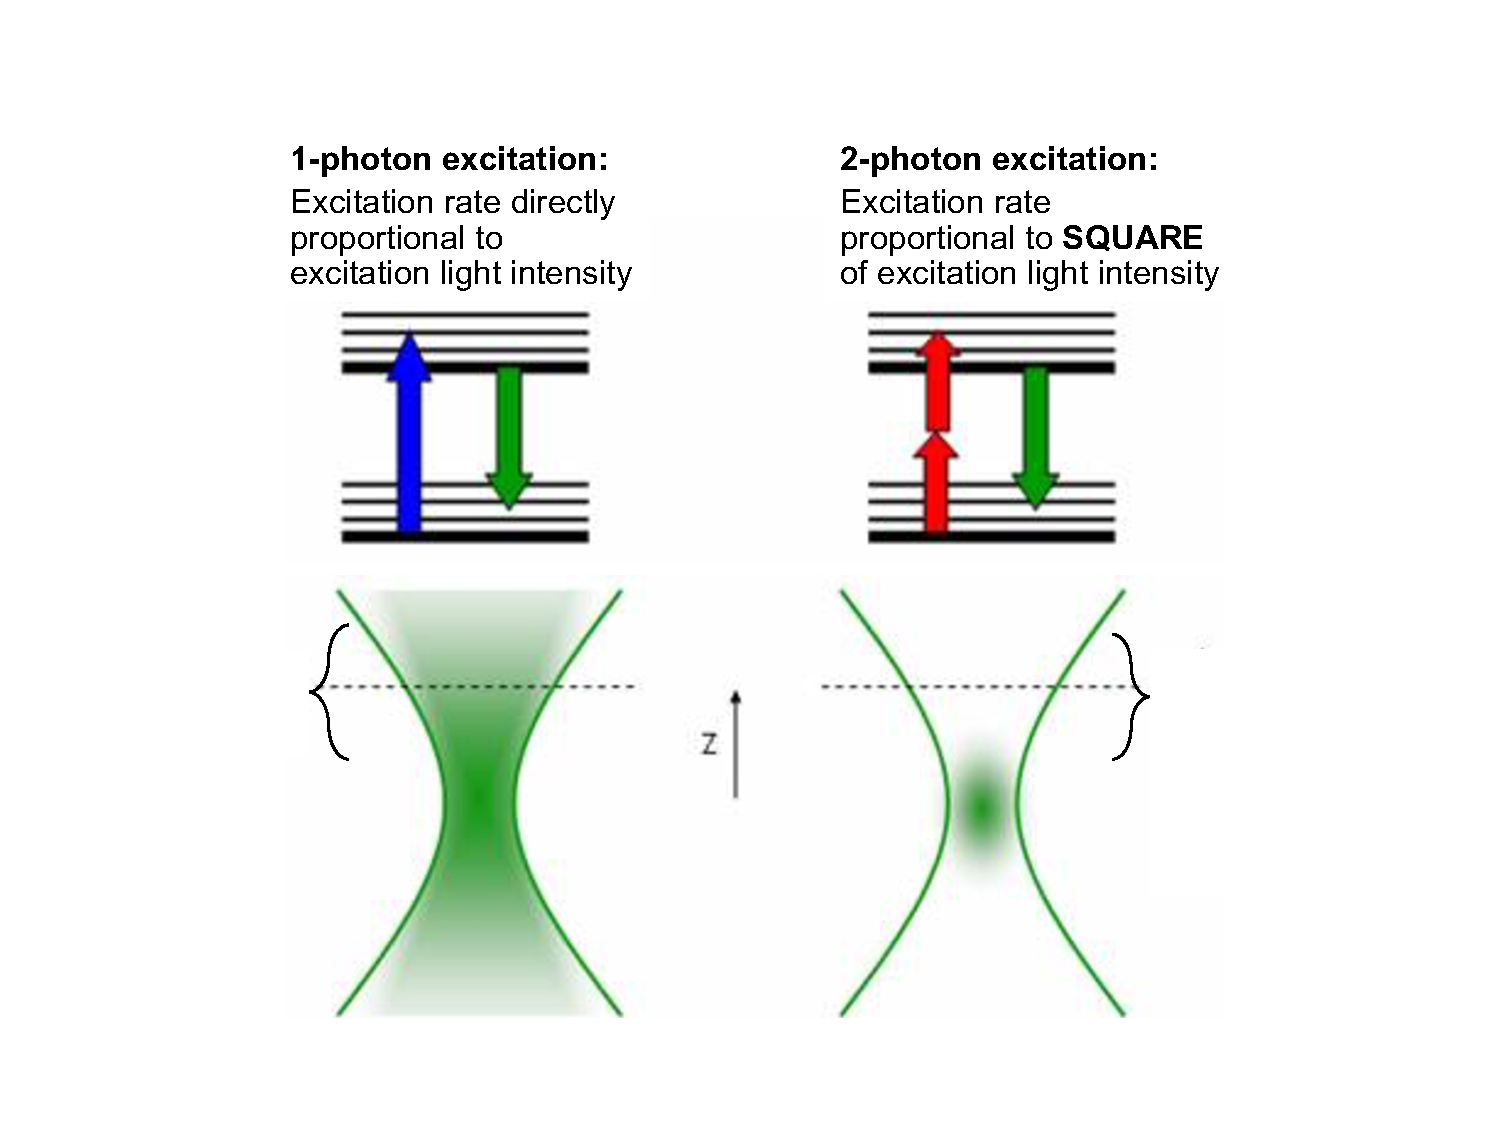
\includegraphics[width=.9\columnwidth]{Detection_2ph_Excitation}
\end{minipage}%
\begin{minipage}{.7\columnwidth}
    \begin{itemize}
        \item[+] wavelength$\uparrow$ $\to$ less absorbing/scattering
        \item[+] photons need to coincide in space and time to excite
        \item[+] No pinhole by detector for 2ph: Collect all the light
        \item[--] low prob. of occurrence i.e. inefficient
        \item[--] ultra-short pulse light source needed
    \end{itemize}
\end{minipage}
